\documentclass[12pt, a4paper, twoside]{article}
\usepackage{titlesec}
\usepackage{calc}
\usepackage{config}
\usepackage{epigraph}
\usepackage{fancyhdr}
\usepackage{csquotes}
\usepackage{hyperref}
\usepackage{notebook}

\title{Mathematical Modelling with Python}
\author{Thien V. Hoang}

\begin{document}
\pagestyle{fancy}
\maketitle
\abstract{Python là ngôn ngữ lập trình bậc cao mã nguồn mở có tính phổ biến cực lớn trong giới công nghệ. Trong trại hè Toán học và Ứng dụng PiMA 2017, chúng ta sẽ tìm hiểu về tính ứng dụng của Python trong nghiên cứu các mô hình toán học từ thực tế. Bài viết giới thiệu Python, các thuật ngữ lập trình, cách cài đặt Jupyter Notebook, và một số vấn đề sẽ được thảo luận tại trại hè. Các bạn chú ý các thuật ngữ tiếng Anh trong ngoặc đơn có thể được sử dụng nhiều lần trên bài viết. Tác giả bài viết không sử dụng hệ điều hành Windows, tuy nhiên cách thực hiện sẽ không quá khác biệt. Các mục được đánh dấu sao (*) trong bài là những mục nâng cao, chuyên sâu, phù hợp hơn với những bạn có background về tin học do đó không yêu cầu các bạn nhập môn lập trình tìm hiểu.\\

\textbf{Lưu ý quan trọng:} Tài liệu này chỉ giới thiệu nhanh về workshop Python sắp tới tại PiMA. Các bạn sẽ được cung cấp thêm các notebook khác để đọc, nghiên cứu, và thí nghiệm.}

\section{Giới thiệu về lập trình}
Lập trình có thể được hiểu là ``hướng dẫn'' cho máy tính của bạn làm theo ý bạn thông qua những câu lệnh. Lập trình có thể được dùng cho nhiều mục đích khác nhau, từ việc tạo ra những ứng dụng và trò chơi trên điện thoại cho đến hệ thống xe tự lái, xa hơn nữa là công cụ tính toán và phân tích trong các trung tâm nghiên cứu về vũ trụ như NASA. Tuy vậy, ở một mức độ cơ bản có thể hiểu lập trình là giải quyết những bài toán (problem solving). Bài toán lớn hơn lại có thể được thiết kế thành những bài toán nhỏ và sau đó ghép các kết quả lại với nhau, giống như một \textbf{kỹ sư}. Bài toán cũng có thể được mô hình theo các công thức giống như các \textbf{nhà toán học} thường làm khi nghiên cứu. Và công việc lập trình cũng đòi hỏi tư duy lập ra những giả thuyết, dự đoán, khả năng kiểm tra lời giải, và quan sát tính chất phức tạp của hệ thống máy tính. Điều này khiến bạn trở thành một \textbf{nhà khoa học máy tính}.

Máy tính chỉ hiểu thông tin ở dạng mã nhị phân. Con người không thể hiểu được. Người ta bắt đầu cho ra những ngôn ngữ bậc thấp đầu tiên như Assembly ở dạng chữ, dễ đọc hơn, rồi từ đó biên dịch ra ngôn ngữ máy. Nhưng sau này nhận thấy ngôn ngữ bậc thấp còn quá phức tạp, khó tiếp cận, khiến cho công nghiệp máy tính phát triển chậm chạp, người ta nghĩ ra ngôn ngữ lập trình bậc cao với cú pháp và từ khóa thân thuộc với con người. Python là một trong số đó.

Lập trình là một công việc rất đơn giản, càng nghiên cứu thì càng thấy sự khó khăn phức tạp. Trong quá trình code các bạn rất dễ gặp lỗi nếu không kiểm soát tốt. Có ba loại lỗi là lỗi cú pháp (syntax), lỗi phát sinh trong thời gian chạy (runtime error), và lỗi trong thuật toán khiến bài toán cho kết quả không mong muốn (semantic error). Nếu so sánh với toán học:
\begin{itemize}
    \item Syntax error: Là những lỗi về cú pháp và cách trình bày như viết sai ký hiệu toán học khiến lời giải trở nên vô nghĩa, không có giá trị. Ví dụ như ký hiệu tính tổng sigma ($\sum$) mà bạn xoay 90 độ viết thành chữ M thì chẳng ai hiểu đó là gì.
    \item Runtime error: Là những lỗi phát sinh trong quá trình bạn giải toán mà bạn quên kiểm soát như vi phạm vào điều kiện xác định làm cho lời giải không còn giá trị. Ví dụ khi giải phương trình, trong một bước nào đó bạn chia hai vế cho một biểu thức mà không nhận ra rằng biểu thức đó sẽ có giá trị bằng 0 tại một số trường hợp. Lúc này lời giải của bạn sẽ có lúc cho ra đáp án, có lúc \textit{không thể} đưa ra đáp án vì sự vi phạm này.
    \item Semantic error: Lỗi này là nguy hiểm nhất và khó sửa nhất. Bạn đã ràng buộc rất tốt ở hai lỗi trên, tức là bạn không sáng tạo ra ký hiệu toán học mới mà cũng đã xét đầy đủ điều kiện xác định. Nhưng cuối cùng lời giải của bạn cho ra kết quả sai. Và bạn phát hiện ra bạn đã vô tình viết ký hiệu $\infty$ thành số 8. Mọi thứ trong lời giải đều hoạt động rất trơn tru, không có lỗi buộc phải dừng, nhưng kết quả lại không như mong muốn.
\end{itemize}

Việc sửa lỗi (debug) là một công việc không mấy dễ chịu đối với lập trình viên. Tuy nhiên giống như các nhà toán học, cảm giác giải được bài toán là cảm giác hưng phấn nhất và khiến cuộc đời trở nên đáng sống hơn bao giờ hết.

\section{Tại sao lại dùng Python?}
\begin{itemize}
    \item Đơn giản, ngắn gọn, dễ đọc, dễ hiểu.
    \item Code linh động: không cần khai báo kiểu dữ liệu của biến hay hàm.
    \item Bộ nhớ đệm được tự động quản lý.
    \item Có hệ thống thư viện khổng lồ (bao gồm cả thư viện từ bên thứ ba), có cộng đồng năng động và rộng lớn.
    \item Python được thông dịch: từng dòng lệnh được dịch và chạy (execute). Tốn ít thời gian phân tích code và dừng ngay ở lệnh bị lỗi giúp dễ debug hơn.
    \item Python là một ngôn ngữ rất mạnh mẽ với rất nhiều hàm và cấu trúc dữ liệu được ``làm sẵn'' khiến cho công việc rất dễ dàng.
\end{itemize}
Tuy nhiên, do từng dòng lệnh được dịch trong lúc chương trình được thực thi (runtime) nên code Python chạy lâu hơn C/C++.
\subsection*{* Các khái niệm khác}
\begin{itemize}
    \item \textbf{CPython:} là một hệ thống xử lý (implementation\footnote{Implementation hàm chỉ tập hợp các cách thức, phương pháp để chuyển đổi code thành ngôn ngữ máy. Trong phần lớn trường hợp implementation là trình biên dịch (compiler) hoặc trình thông dịch (interpreter) hoặc có sự phối hợp của cả hai.}) code Python chính thức của Python Software Foundation. CPython có nền tảng là ngôn ngữ C, thường được đề cập để phân biệt với các implementations khác như Jython (nền tảng là Java). Trong phạm vi tài liệu này, mọi đề cập đến `Python' xin được ngầm hiểu là `CPython', trừ khi được nhắc cụ thể.
    \item \textbf{Cython:} là một phần mềm giúp chuyển code Python sang code C để chạy code nhanh hơn (transpiler).
    \item \textbf{Just-in-time (JIT) compiler:} là trình biên dịch chạy trong runtime giúp tìm ra các đoạn \textit{bytecode} được interpreted quá nhiều lần để compile hẳn chúng ra ngôn ngữ máy để tiết kiệm thời gian chạy chương trình. JIT can thiệp được vào các thông tin trong runtime mà một compiler bình thường không làm được để tối ưu chương trình tốt hơn, chẳng hạn như tự động \textit{inline} một hàm. \textbf{PyPy} là một dự án JIT vừa phát triển gần đây của ngôn ngữ Python giúp code có thể chạy nhanh hơn Python thông thường một cách đáng kể.
\end{itemize}
\section{* Các khái niệm cơ bản trong Python}
\begin{itemize}
    \item \textbf{Package:} Một gói thư viện mở rộng cho Python có thêm nhiều tính năng để hoạt động tốt hơn và để người lập trình code nhanh hơn. Package có thể được phân phối (distribute) bởi Python Software Foundation (có sẵn khi cài Python) hoặc bên thứ ba (third party) như scipy, numpy, etc. (phải cài thêm thông qua \textit{pip}).
    \item \textbf{Module:} Là thành phần con của Package. Một module có thể là một folder bao gồm nhiều module khác hoặc là một file, nhưng không nhỏ hơn một file. Thông thường người ta không quá khắt khe về việc phân biệt package và module.
    \item \textbf{Class:} Bên trong một module được định nghĩa nhiều class khác nhau. Ý nghĩa cơ bản của class là tạo ra một đối tượng, một kiểu dữ liệu mới bao gồm những \textit{thuộc tính} và \textit{hàm} tự định nghĩa hoặc tái định nghĩa để dễ kiểm soát, dễ theo dõi khi lập trình.
    \item \textbf{Function:} Một đoạn mã được copy \& paste nhiều lần có thể được nhóm lại và định nghĩa thành một hàm để code nhanh hơn và linh động hơn qua các \textit{tham số} (parameters).
    \item \textbf{pip:} Là một package manager giúp bạn cài đặt thêm những package mới theo nhu cầu, thông qua lệnh \texttt{pip install <package>} trên Terminal. Chữ `pip' là viết tắt đệ quy của câu ``Pip install packages'' (Source: Wikipedia).
\end{itemize}
\section{Làm sao để sử dụng Python?}
Trên macOS có cài đặt sẵn Python 2. Trên Ubuntu có cài đặt sẵn Python 2 và Python 3. Để kiểm tra mình có Python trên máy chưa, vào Terminal (hoặc Command Prompt trên Windows) gõ lệnh \texttt{python --version} để xem có báo lỗi hay không. \textbf{Trong trại hè lần này khuyến khích các bạn dùng Python 3.}

Sau đây là các cách khác nhau để chạy code Python:
\begin{itemize}
    \item Code trên file: Mở một file bằng editor (e.g. Notepad, Sublime, Atom, etc.) tùy ý và gõ code ở đó. Lưu lại thành một file có đuôi (extension) là \texttt{.py}. Vào Terminal chạy lệnh:\\
    \texttt{\$ python file-name.py}
    \item Chạy từng câu lệnh một trên Terminal: Bằng cách gõ lệnh \texttt{python} trong Terminal, nó sẽ mở ra một process Python. Gõ từng lệnh một và enter sẽ cho ra kết quả.
    \item \textbf{Jupyter Notebook:} (recommended) Một môi trường lập trình Python có nền tảng HTML. Trong một notebook, bạn có thể viết code vào các `khối' (cell) code và chạy cell đó một cách trực quan. Các khối khi nhận lệnh chạy sẽ nối đuôi nhau thực thi trong một process Python. Ngoài ra các phép tính toán và tài liệu có thể được trình bày tường minh trong các loại cell khác để bổ sung thông tin cho code. Có hỗ trợ viết bằng \LaTeX\ và export notebook thành file \LaTeX\ để các bạn đưa vào bài nghiên cứu của mình.
\end{itemize}
\subsection*{Hướng dẫn cài đặt Jupyter Notebook}
Trong Terminal / Command Prompt bạn hãy gõ lần lượt các lệnh sau (phải chờ lệnh trước kết thúc mới tới lệnh sau):
\begin{verbatim}
    pip3 install jupyter
    jupyter notebook
\end{verbatim}
Sau đó vào trình duyệt web truy cập địa chỉ \texttt{localhost:8888}, bạn sẽ thấy các thư mục trên máy tính của bạn. Lần lượt tìm đến thư mục chứa notebook (là file có đuôi \texttt{.ipynb}) và mở lên.
\begin{figure}[htb]
    \centering
    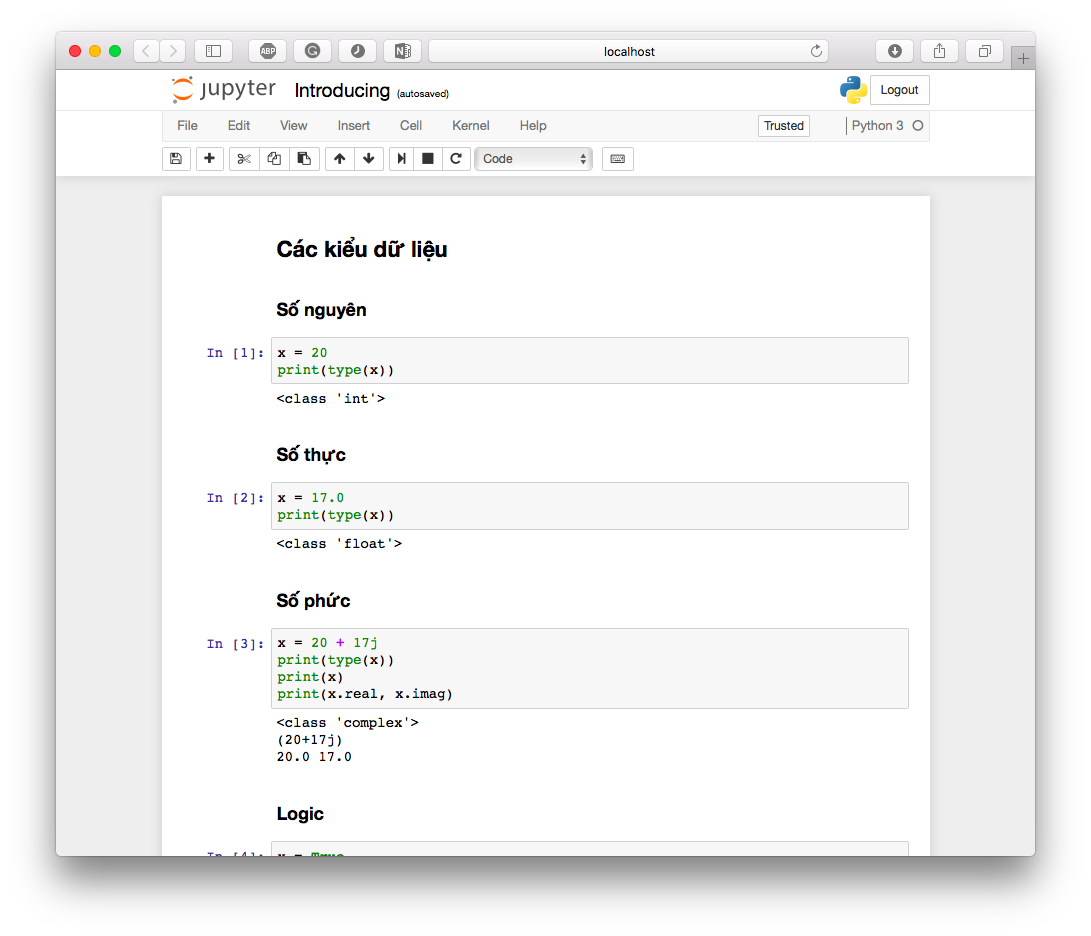
\includegraphics{jupyter_nb.png}

\end{figure}

\section{Kiến thức căn bản về ngôn ngữ Python}
Khác với sự gò bó của C++ và Java, chỉ với một cú pháp nhỏ trong Python lại sinh ra rất nhiều phép tính và thao tác đến mức không thể kể hết trong tài liệu này. Tuy nhiên, để giới thiệu các bạn đến với Python, sau đây là những kiến thức không thể thiếu:
\begin{itemize}
    \item Các kiểu dữ liệu: \texttt{int, float, complex, bool, str, list, dict, tuple}. Cách ép kiểu dữ liệu.
    \item Các phép toán cơ bản (cộng, trừ, ...). Thao tác thêm, bớt, truy xuất phần tử, hàm sắp xếp. Thao tác cắt mảng.
    \item Vòng lặp và rẽ nhánh.
    \item Cách viết một hàm, một class.
\end{itemize}
\section{Giới thiệu các package}
\subsection{\texttt{numpy}}
\texttt{numpy} thường được sử dụng để tạo các object mảng đa chiều (multi-dimensional array). Mặc dù về cơ bản, Python đã có hỗ trợ mảng đa chiều (list \& nested-list) nhưng:
\begin{itemize}
    \item Trong Python, mảng không có sự thống nhất. Các phần tử có thể chứa bất kỳ dữ liệu kiểu gì cũng được. Mặc dù nghe có vẻ là một ``tính năng'' linh động nhưng trong nhiều trường hợp việc có một cấu trúc dữ liệu (data structure) ổn định và thống nhất lại được ưa chuộng hơn.
    \item Do tính chất nói trên của dữ liệu nên các thao tác với mảng được tối ưu rất nhiều qua việc tích hợp với C/C++ và Fortran.
    \item \texttt{numpy} hỗ trợ nhiều phép tính với ma trận như tìm ma trận nghịch đảo, tìm tích vô hướng giữa hai ma trận, etc.
\end{itemize}
Chúng ta bắt đầu với \texttt{numpy} bằng cách \texttt{import} thư viện này vào file Python (hoặc kernel) đang code.

Các chủ đề được thảo luận:
\begin{itemize}
    \item Giới thiệu về array và matrix.
    \item Các phép tính với array và matrix.
    \item Các thông số quan trọng khi thống kê dữ liệu trong array.
    \item Pass by reference.
    \item Chọn lọc dữ liệu bằng cách dùng mặt nạ.
    \item Vector hóa một hàm
\end{itemize}
\subsection{Vẽ đồ thị}
Sử dụng thư viện \texttt{matplotlib} để vẽ các dạng đồ thị thông qua dữ liệu hoặc hàm. Định dạng đồ thị, bố trí các đối tượng trên hình ảnh.
\subsection{\texttt{scipy}}
\texttt{scipy} là một thư viện được xây dựng trên nền tảng \texttt{numpy}, cung cấp một lượng lớn các chức năng phục vụ tính toán khoa học. Các phần được giới thiệu trong trại hè bao gồm:
\begin{itemize}
    \item \texttt{scipy.integrate}: Tích phân và phương trình vi phân
    \item \texttt{scipy.linalg}: Hệ phương trình tuyến tính và ma trận thưa
    \item \texttt{scipy.optimize}: Tìm các cực trị của hàm số
    \item \texttt{scipy.interpolate}: Tìm xu hướng biến động của dữ liệu bị nhiễu
\end{itemize}
\subsection{\texttt{sympy}}
\texttt{sympy} là một thư viện toán học trên Python hỗ trợ từ đại số đến hình học và xa hơn là vật lý, thống kê, mã hóa. Các phần sau đây sẽ được giới thiệu:
\begin{itemize}
    \item Tính toán cơ bản
    \item Biến đổi biểu thức toán học
    \item Tính đạo hàm, nguyên hàm của hàm số
    \item Giải phương trình
\end{itemize}
\end{document}
